%%%%%%%%%%%%%%%%%%%%%%%%%%%%%%%%%%%%%%%%%
% Beamer Presentation
% LaTeX Template
% Version 1.0 (10/11/12)
%
% This template has been downloaded from:
% http://www.LaTeXTemplates.com
%
% License:
% CC BY-NC-SA 3.0 (http://creativecommons.org/licenses/by-nc-sa/3.0/)
%
%%%%%%%%%%%%%%%%%%%%%%%%%%%%%%%%%%%%%%%%%

%----------------------------------------------------------------------------------------
%	PACKAGES AND THEMES
%----------------------------------------------------------------------------------------

\documentclass{beamer}

\mode<presentation> {

% The Beamer class comes with a number of default slide themes
% which change the colors and layouts of slides. Below this is a list
% of all the themes, uncomment each in turn to see what they look like.

%\usetheme{default}
%\usetheme{AnnArbor}
%\usetheme{Antibes}
%\usetheme{Bergen}
%\usetheme{Berkeley}
%\usetheme{Berlin}
%\usetheme{Boadilla}
%\usetheme{CambridgeUS}
%\usetheme{Copenhagen}
%\usetheme{Darmstadt}
%\usetheme{Dresden}
%\usetheme{Frankfurt}
%\usetheme{Goettingen}
%\usetheme{Hannover}
%\usetheme{Ilmenau}
%\usetheme{JuanLesPins}
%\usetheme{Luebeck}
\usetheme{Madrid}
%\usetheme{Malmoe}
%\usetheme{Marburg}
%\usetheme{Montpellier}
%\usetheme{PaloAlto}
%\usetheme{Pittsburgh}
%\usetheme{Rochester}
%\usetheme{Singapore}
%\usetheme{Szeged}
%\usetheme{Warsaw}

% As well as themes, the Beamer class has a number of color themes
% for any slide theme. Uncomment each of these in turn to see how it
% changes the colors of your current slide theme.

%\usecolortheme{albatross}
%\usecolortheme{beaver}
%\usecolortheme{beetle}
%\usecolortheme{crane}
%\usecolortheme{dolphin}
%\usecolortheme{dove}
%\usecolortheme{fly}
%\usecolortheme{lily}
%\usecolortheme{orchid}
%\usecolortheme{rose}
%\usecolortheme{seagull}
%\usecolortheme{seahorse}
%\usecolortheme{whale}
%\usecolortheme{wolverine}

%\setbeamertemplate{footline} % To remove the footer line in all slides uncomment this line
%\setbeamertemplate{footline}[page number] % To replace the footer line in all slides with a simple slide count uncomment this line

%\setbeamertemplate{navigation symbols}{} % To remove the navigation symbols from the bottom of all slides uncomment this line
}

\usepackage{graphicx} % Allows including images
\usepackage{booktabs} % Allows the use of \toprule, \midrule and \bottomrule in tables

%----------------------------------------------------------------------------------------
%	TITLE PAGE
%----------------------------------------------------------------------------------------

\title[Investigating spillover effects]{Testing for Network Effects in Field Experiments} % The short title appears at the bottom of every slide, the full title is only on the title page
\subtitle{Examples from Legislative Studies}

\author{Sayali Phadke\inst{1} \and Bruce A. Desmarais\inst{2}}
% - Give the names in the same order as the appear in the paper.
% - Use the \inst{?} command only if the authors have different
%   affiliation.

\institute[Pennsylvania State University] % (optional, but mostly needed)
{
  \inst{1}%
  PhD student\\
  Department of Statistics
  \and
  \inst{2}%
  Associate Professor\\
  Department of Political Science}

% - Use the \inst command only if there are several affiliations.
% - Keep it simple, no one is interested in your street address.

\date{Political Networks 2016}
% - Either use conference name or its abbreviation.
% - Not really informative to the audience, more for people (including
%   yourself) who are reading the slides online

%\subject{Theoretical Computer Science}
% This is only inserted into the PDF information catalog. Can be left
% out. 

% If you have a file called "university-logo-filename.xxx", where xxx
% is a graphic format that can be processed by latex or pdflatex,
% resp., then you can add a logo as follows:

% \pgfdeclareimage[height=0.5cm]{university-logo}{university-logo-filename}
% \logo{\pgfuseimage{university-logo}}

% Delete this, if you do not want the table of contents to pop up at
% the beginning of each subsection:
%\AtBeginSubsection[]
%{
%  \begin{frame}<beamer>{Outline}
%    \tableofcontents[currentsection,currentsubsection]
%  \end{frame}
%}

\begin{document}

\begin{frame}
\titlepage % Print the title page as the first slide
\end{frame}

\begin{frame}
\frametitle{Overview} % Table of contents slide, comment this block out to remove it
\tableofcontents % Throughout your presentation, if you choose to use \section{} and \subsection{} commands, these will automatically be printed on this slide as an overview of your presentation
\end{frame}

%----------------------------------------------------------------------------------------
%	PRESENTATION SLIDES
%----------------------------------------------------------------------------------------


%%%%%%%% Slide: overview
% Section and subsections will appear in the presentation overview
% and table of contents.
\section{Motivation}

%\subsection{First Subsection}

%\begin{frame}{First Slide Title}{Optional Subtitle}
%  \begin{itemize}
%  \item {
%    My first point.
%  }
%  \item {
%    My second point.
%  }
%  \end{itemize}
%\end{frame}

%\subsection{Second Subsection}

% You can reveal the parts of a slide one at a time
% with the \pause command:
%\begin{frame}{Second Slide Title}
%  \begin{itemize}
%  \item {
%    First item.
%    \pause % The slide will pause after showing the first item
%  }
%  \item {   
%    Second item.
%  }
  % You can also specify when the content should appear
  % by using <n->:
%  \item<3-> {
%    Third item.
%  }
%  \item<4-> {
%    Fourth item.
%  }
  % or you can use the \uncover command to reveal general
  % content (not just \items):
%  \item<5-> {
%    Fifth item. \uncover<6->{Extra text in the fifth item.}
%  }
%  \end{itemize}
%\end{frame}

%\subsection{Another Subsection}

% Placing a * after \section means it will not show in the
% outline or table of contents.
\section*{Summary}


%%%%%%%% Slide 1
\begin{frame}
\frametitle{Motivation: Causal diagram}
Several factors impact the effect of treatment on the outcome
\begin{figure}
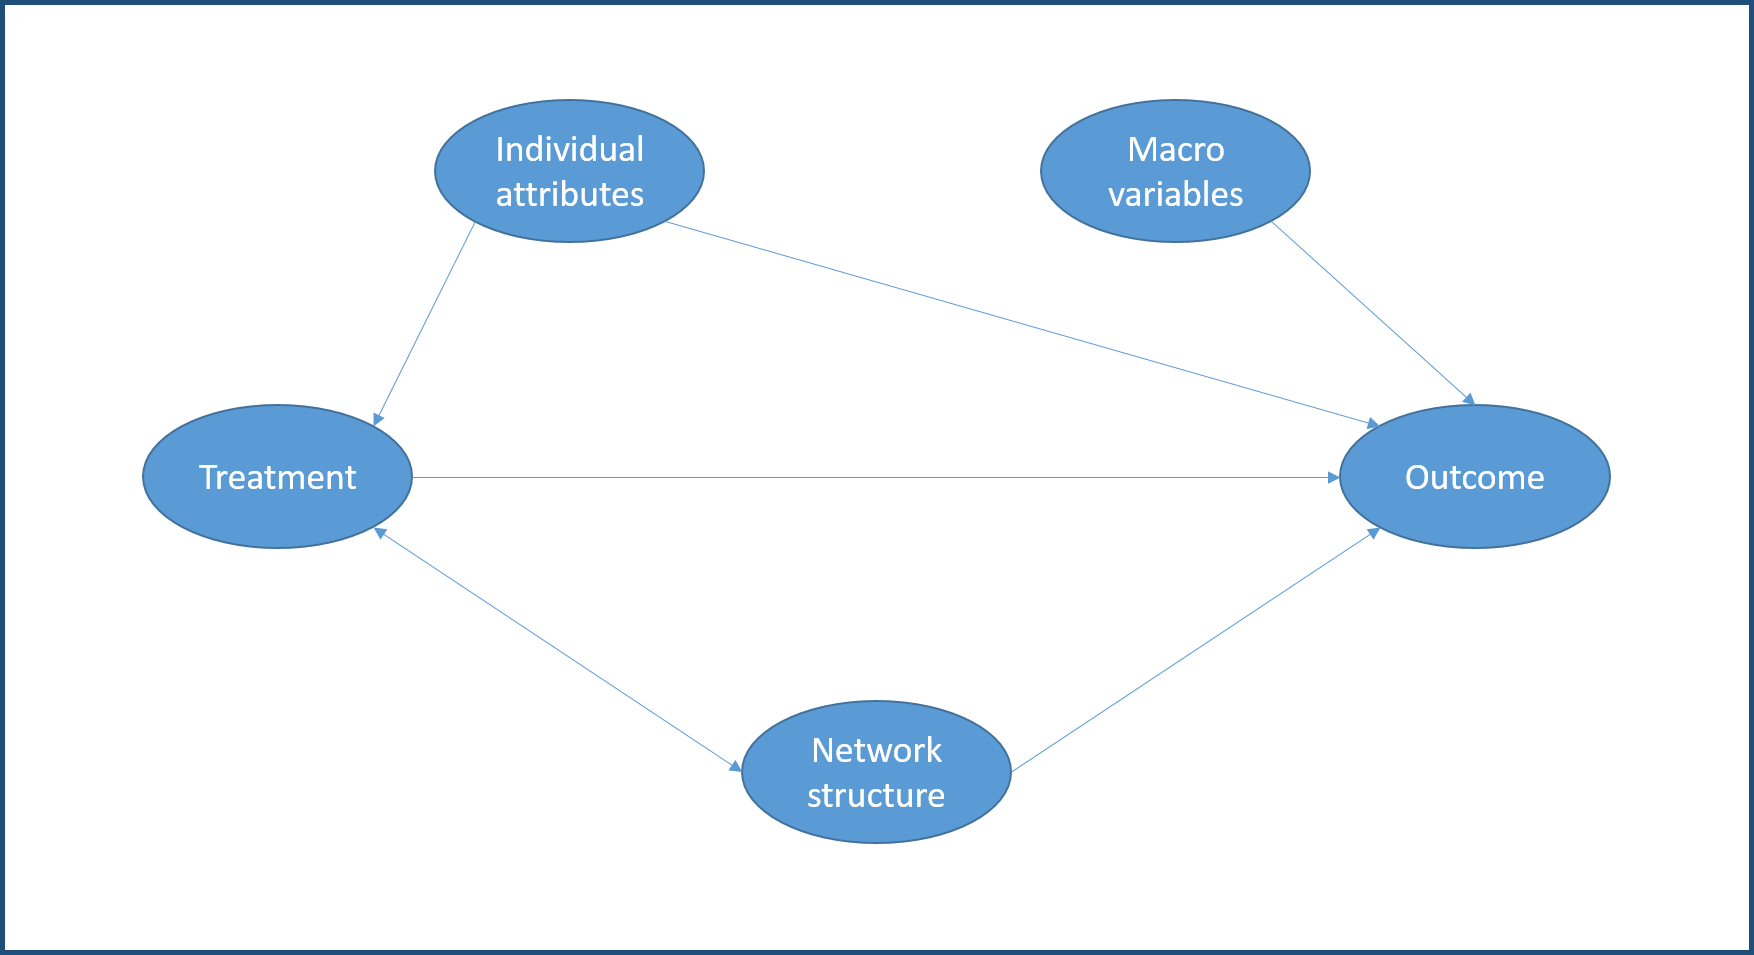
\includegraphics[width=0.8\linewidth]{Causal_diagram_1.png}
\end{figure}
\end{frame}


%%%%%%%% Slide 2: continuation of 1
\begin{frame}
\frametitle{Motivation: Causal diagram}
Field experiments eliminate systematic treatment assignment, but not the effect of network
\begin{figure}
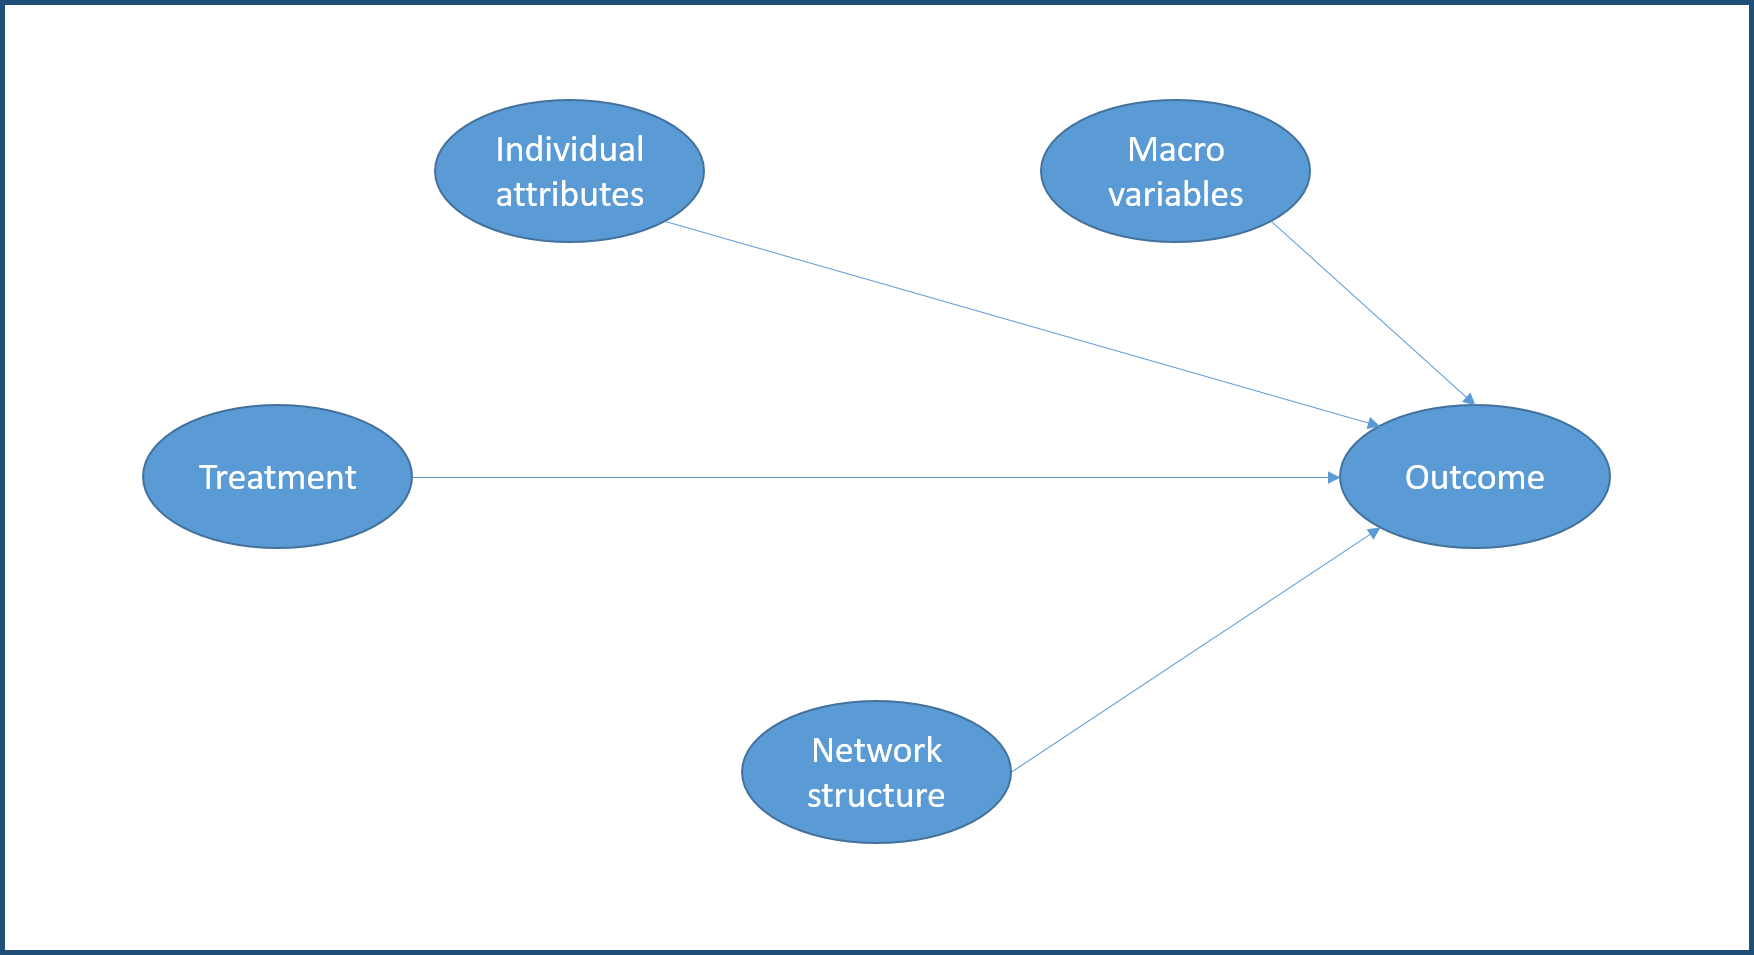
\includegraphics[width=0.8\linewidth]{Causal_diagram_2.png}
\end{figure}
\end{frame}


%%%%%%%% Slide 3: network plot
\begin{frame}
\frametitle{Motivation: Network plot}
\begin{figure}
\includegraphics[width=0.8\linewidth]{Dummy_network_plot.png}
\end{figure}

\vspace{-0.5cm}
\begin{block}{Stable Unit Treatment Value Assumption (SUTVA)}
Assumption that the treatment status of unit does not affect the outcome of another.
\end{block}
\end{frame}


%%%%%%%% Slide 4: research objectives
\begin{frame}
\frametitle{Research objectives}
\begin{itemize}
\item Model spillover of treatment effect via network structures.
\item Examine how inferences depend upon the specification of the network and spillover
structure.
\item Evaluate the models using data from field experiments on US State legislatures.
\end{itemize}
\end{frame}


%%%%
\section{Methodology}
%%%%

%%%%%%%% Slide 5: Bowers method
\begin{frame}
\frametitle{Method: Review}
\begin{itemize}

\item Method for modeling and testing for interference effects using non-parametric test under Fisher's inference framework (Bowers, Fredrickson and Panagopoulos (2012))
\item Sharp null hypothesis of no effects assumed
\item Spillover depends on the number of treated neighbors
\item Spillover model specification includes separate parameters for direct and indirect treatment effect
\item Kolmogorov-Smirnov (KS) test used to compare treatment and control group under a large number of permutations of treatment assignment

\end{itemize}
\end{frame}


%%%%%%%% Slide 6: Salient dimensions
\begin{frame}
\frametitle{Method: Extensions}

%\begin{columns}[c]

%	\column{.65\textwidth}
	\begin{itemize}
	
	\item \textbf{Neighborhood specification:}
		\begin{itemize}
		\item Effect from all units
		\item Effect from k-nearest neighbors 
		\end{itemize}
		
	\item \textbf{Diffusion model specification:}
		\begin{itemize}
		\item Distance from the nearest treated node
		\item Number/proportion of treated neighbors
		\item Form of spread (linear or non-linear)
		\end{itemize}
%	\end{itemize}

%	\column{.5\textwidth}
%	\begin{itemize}
	\item \textbf{Network selection:}
		\begin{itemize}
		\item Ideological network
		\item Committee network
		\item Co-sponsorship network
		\item Geographical network network
		\end{itemize}
					
	\item \textbf{Test statistic selection:}
		\begin{itemize}
		\item Kolmogorov-Smirnov test
		\item Anderson-Darling test
		\item Mann-Whitney U test
		\item Control Median test
		\end{itemize}
	\end{itemize}

%\end{columns}
\end{frame}


%%%%
\section{Applications}
%%%%

%%%%%%%% Slide 6: Salient dimensions
\begin{frame}
\frametitle{Application: Coppock (2014)}
\begin{columns}[c]

\column{.55\textwidth}
\begin{figure}
\centering
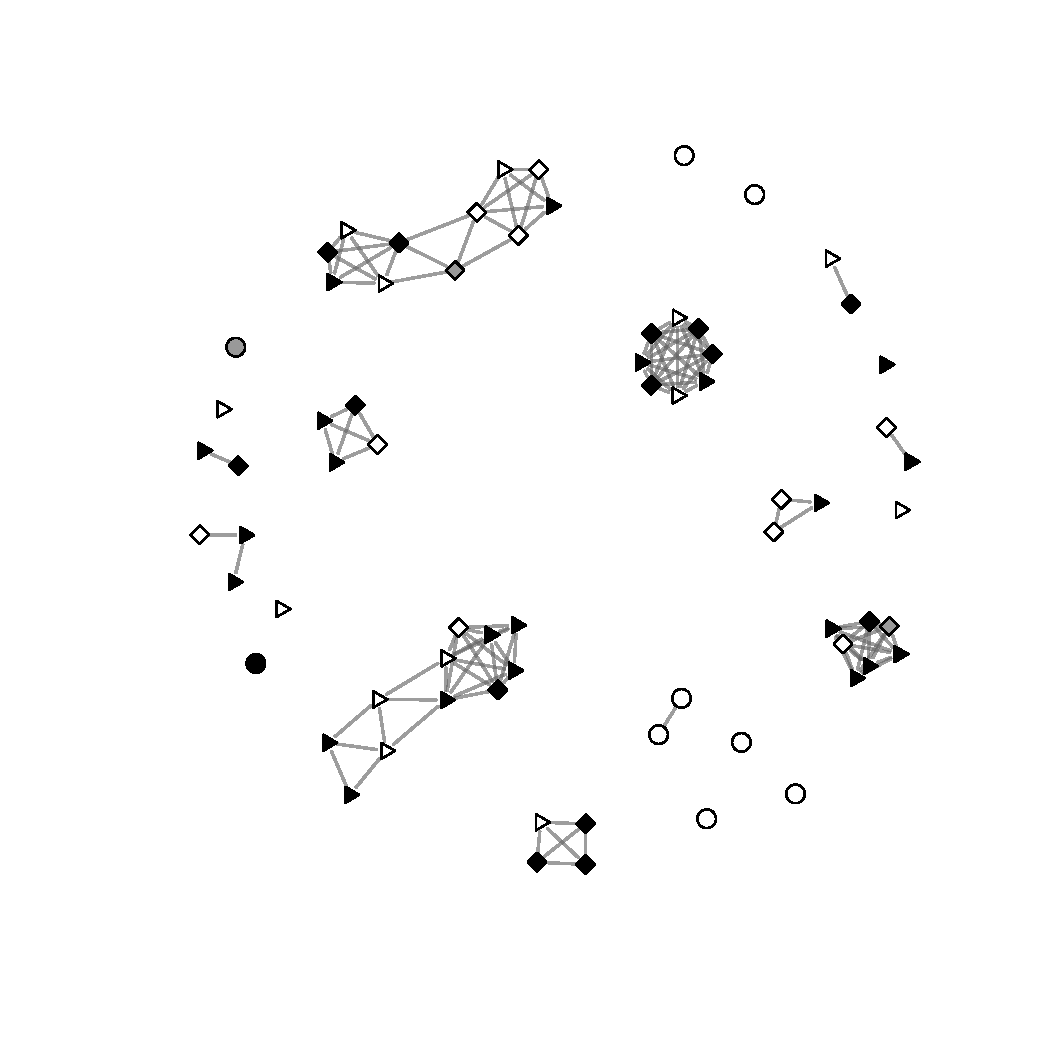
\includegraphics[scale=0.3]{Coppock_ideological_net.pdf}
\caption{Ideological network: Butler, Nickerson et. al. (2011)}
\end{figure}

\column{.55\textwidth}
\begin{figure}
\centering
\includegraphics[scale=0.3]{Coppock_pvalues_temp.pdf}
\caption{TEMP: Replication of Coppock (2014)}
\end{figure}

\end{columns}
\end{frame}


%%%%%%%% Slide 7: Coppock extensions 1
\begin{frame}
\frametitle{Application: Extension of Coppock (2014) analysis 1}
Plots are temporary. Will be changed before the conference. Knn specifications
	\begin{figure}
	\centering
	\begin{tabular}{cc}
	\includegraphics[scale=0.2]{Coppock_pvalues_3nn.pdf} &
	\includegraphics[scale=0.2]{Coppock_pvalues_5nn.pdf} \\ 
	\includegraphics[scale=0.2]{Coppock_pvalues_8nn.pdf} &
	\includegraphics[scale=0.2]{Coppock_pvalues_12nn.pdf} \\ 
	\end{tabular}
	\caption{p-values: Nearest neighbor specification}
	\end{figure}
\end{frame}


%%%%%%%% Slide 8: Coppock extensions 2
\begin{frame}
\frametitle{Application: Extension of Coppock (2014) analysis 2}
Plots are temporary. Will be changed before the conference. Committee network
	\begin{figure}
	\centering
	\begin{tabular}{cc}
	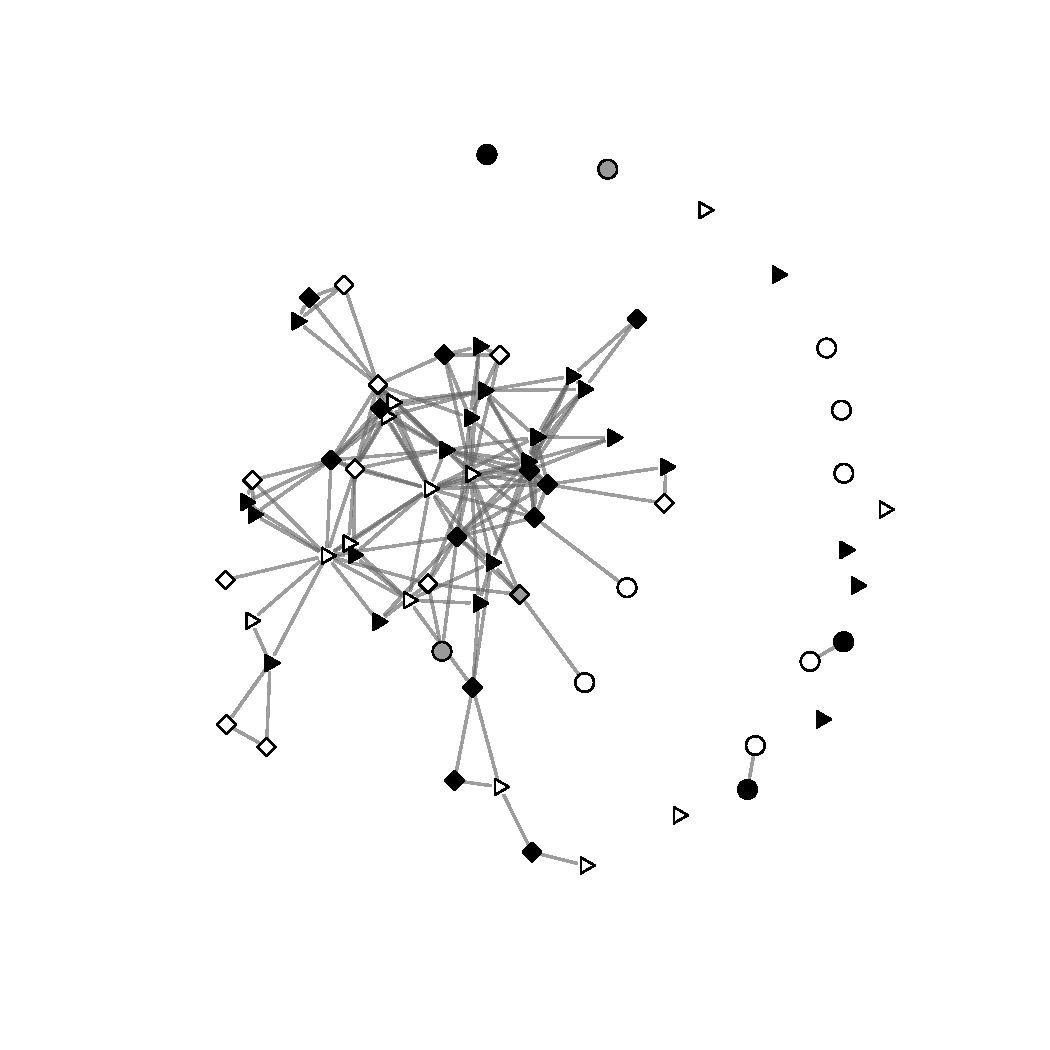
\includegraphics[scale=0.3]{Coppock_nm_committee_net.pdf} &
	\includegraphics[scale=0.3]{Coppock_pvalues_committee.pdf} \\ 
	\end{tabular}
	\caption{p-values: Committee network of New Mexico legislators}
	\end{figure}
\end{frame}


%%%%%%%% Slide 9: Bergan replication
\begin{frame}
\frametitle{Application: Bergan and Cole (2015)}
Include a network plot and replication p-value plot for Bergan
%	\begin{figure}
%	\centering
%	\begin{tabular}{cc}
%	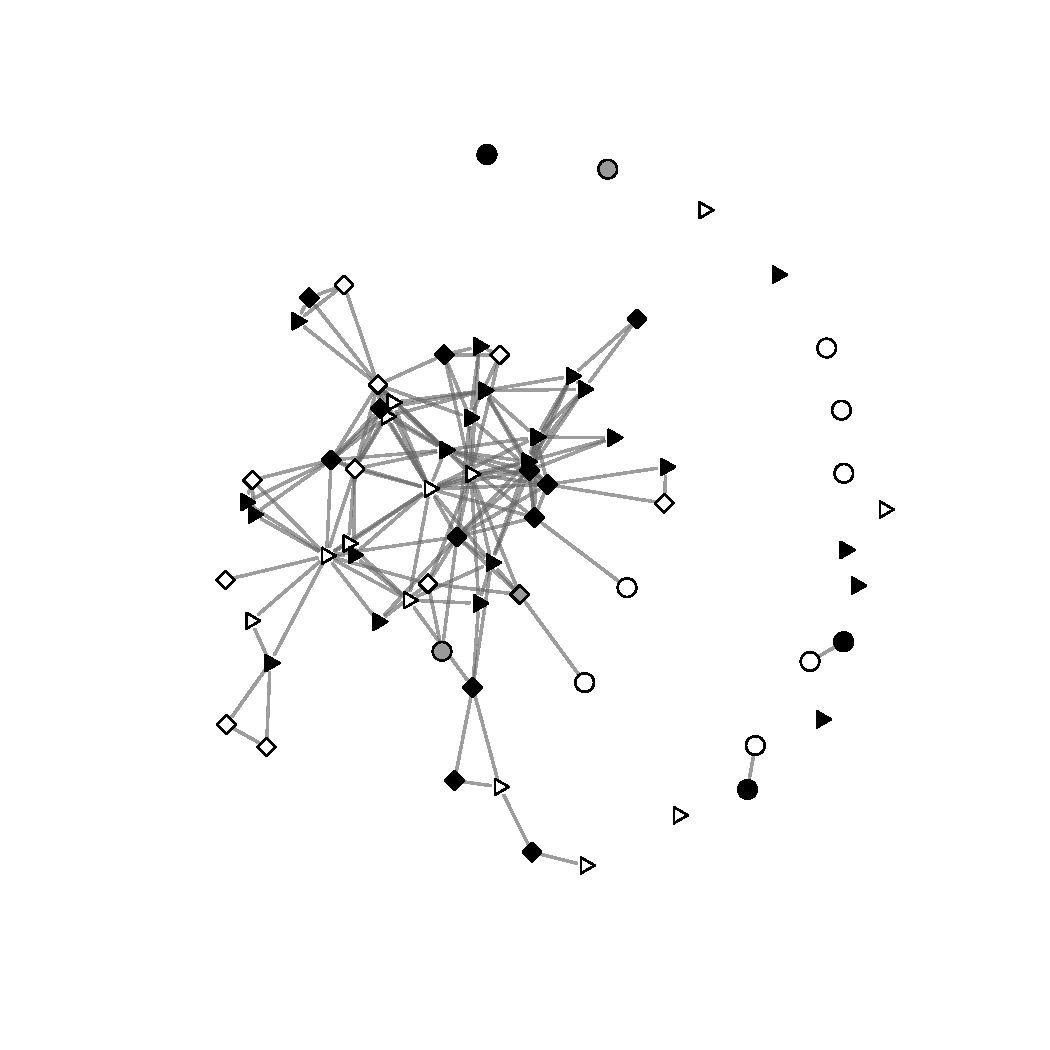
\includegraphics[scale=0.3]{Coppock_nm_committee_net.pdf} &
%	\includegraphics[scale=0.3]{Coppock_pvalues_committee.pdf} \\ 
%	\end{tabular}
%	\caption{p-values: Committee network of New Mexico legislators}
%	\end{figure}
\end{frame}


%%%%
\section{Final remarks}
%%%%

%%%%%%%% Slide 11: Summary and next steps
\begin{frame}{Summary}
  \begin{itemize}
  \item
    Many domains of political science studies interactive social groups and interference must be modeled in analyzing experiments conducted on them
  \item
    Several dimensions must be considered in specifying the model for interference and drawing inferences from the same
  \item
    This analysis can be used to perform power calculations and create optimal experimental design
  \end{itemize}
  
  \begin{itemize}
  \item
    Next steps
    \begin{itemize}
    \item Replicate the Brockman (2013) study that includes legislators from multiple states
    \item Extend replications along salient dimensions
    \item Model a mixture of networks instead of considering a single network
    \end{itemize}
  \end{itemize}
\end{frame}


%%%%%%%% Slide 12: Last slide
\begin{frame}
\Huge{\centerline{Thank you}}
\Huge{\centerline{Questions?}}
\end{frame}


\end{document} 